\documentclass[conference,compsoc]{IEEEtran}
\usepackage{amsmath,amssymb,amsthm}
\usepackage{graphicx}
\graphicspath{{figs/}}
\usepackage{booktabs}
\usepackage{multirow}
\usepackage[hidelinks]{hyperref}
\usepackage{cite}
\usepackage{xcolor}
\usepackage{tikz}
\usetikzlibrary{positioning,arrows.meta}
\newtheorem{proposition}{Proposition}
\newtheorem{corollary}{Corollary}
\newcommand{\ket}[1]{\lvert #1\rangle}
\newcommand{\ev}[1]{\langle #1\rangle}

\begin{document}

\title{Entanglement Does Not Pay (Yet): Noise-Invariant Quantum Features for Fraud Detection, Proven and Measured on IBM Heron Hardware}

\author{\IEEEauthorblockN{Anonymous Authors}\IEEEauthorblockA{Submission under double-blind review}}

\maketitle

\begin{abstract}
Quantum feature maps are routinely proposed for financial fraud detection, yet it is unclear what hardware noise does to the features and whether entanglement is worth its cost. We study expectation-value features $\ev{Z_i}$ of Qiskit's Z, ZZ and Pauli feature maps, fed to XGBoost, an MLP and an RBF-SVM, on one real and two synthetic fraud datasets under a leakage-free protocol at the original fraud prevalence. We prove that for product (unentangled) maps, any noise composed of phase-covariant single-qubit channels---including non-unital amplitude damping and $T_1/T_2$ relaxation---plus readout error acts on each feature as an exact affine map $\ev{Z_i}\mapsto\alpha_i+\beta_i\ev{Z_i}$. Consequently, standardized classifiers are exactly noise-invariant and gate noise only multiplies the required shot budget by $1/\beta^2$. We confirm the law to $10^{-15}$ in simulation and on two IBM Heron processors (360 physical qubits, 3 datasets), where measured features follow it to within shot noise and fraud-detection AUC matches ideal features sampled with the same number of shots. For the entangling ZZ map, the retained signal decays as $\beta\approx\beta_0\eta^{g}$ in the number $g$ of two-qubit gates per qubit, with $\eta=0.990$ on hardware and $0.965$/$0.994$ for our superconducting/trapped-ion models; entangling maps need up to two orders of magnitude more shots. No quantum representation beats using all classical features (largest gain $+0.002$ AUC), and the few hybrid gains are reproduced by matched random Fourier features. On current hardware, the robust quantum features are exactly the classically simple ones.
\end{abstract}

\begin{IEEEkeywords}
Quantum machine learning, quantum feature maps, hardware noise, fraud detection, superconducting and trapped-ion qubits, benchmarking
\end{IEEEkeywords}

\section{Introduction}
Payment fraud is rare (0.1--1\% of transactions), costly and adversarial, which makes it a recurring showcase for quantum machine learning (QML): data are encoded by a parameterized circuit $U_\phi(x)$, and either a kernel or measured observables feed a classifier~\cite{havlicek2019,schuld2019,grossi2022}. Two questions are usually left open. \emph{(i) What does hardware noise do to quantum features?} Most studies report noiseless or lightly-noisy simulations. \emph{(ii) Does entanglement in the feature map pay for its cost?} Entangling gates are the dominant error source on every current platform, and large-scale benchmarks have found that classical baselines often match or beat QML models~\cite{bowles2024}.

We answer both questions for the simplest, most deployable quantum representation (Fig.~\ref{fig:pipeline}): the vector of single-qubit expectation values $z(x)=[\ev{Z_1},\dots,\ev{Z_k}]$ after a feature map, used as input to strong classical classifiers. Our contributions are:
\begin{enumerate}
\item \textbf{An exact noise law for product maps.} For the unentangled Z feature map, any noise built from phase-covariant single-qubit channels and readout error transforms every feature affinely (Proposition~1). Hence standardized classifiers are \emph{exactly} invariant to gate noise, and noise acts only as a shot-budget multiplier $1/\beta^2$ (Corollaries~1--2).
\item \textbf{A hardware-validated cost law for entanglement.} Measured on two IBM Heron devices and simulated for superconducting- and trapped-ion-like models, the signal retained by the ZZ map decays geometrically, $\beta\approx\beta_0\eta^{g}$, in the number of two-qubit gates per qubit.
\item \textbf{A leakage-free benchmark} on one real and two synthetic fraud datasets with three classifiers, three seeds and original-prevalence test sets, including a hybrid test with a matched classical control. Quantum features never beat classical ones.
\item \textbf{Practical rules and pitfalls}: an 11$\times$ cheaper feature selection that finds the exhaustive optimum in 75\% of cases, and three silent failure modes of standard feature maps.
\end{enumerate}

\section{Related Work}
Quantum-enhanced feature spaces and their kernel interpretation were introduced in~\cite{havlicek2019,schuld2019}; for fraud detection, \cite{grossi2022} combined quantum feature selection with QSVMs on hardware-scale problems. Noise in quantum kernels has been analysed mainly for \emph{global depolarizing} noise, which rescales kernel values and can be absorbed by regularization~\cite{wang2021kernels,heyraud2022}; with depth and qubit number, kernels and features may also concentrate exponentially~\cite{thanasilp2024}. Huang et al.~\cite{huang2021} showed that classical models with access to data can rival quantum models, and Bowles et al.~\cite{bowles2024} found that out-of-the-box classical baselines systematically match QML benchmarks. Cerezo et al.~\cite{cerezo2025} argue that structures making variational models trainable often make them classically simulable. We complement these works with (a) an exact per-feature law for \emph{non-unital} noise plus readout, extended to the full learning pipeline including feature selection, (b) direct hardware measurements of the feature distortion, and (c) an empirical per-gate cost law for entangling maps.

\section{Methods}

\begin{figure}[t]
\centering
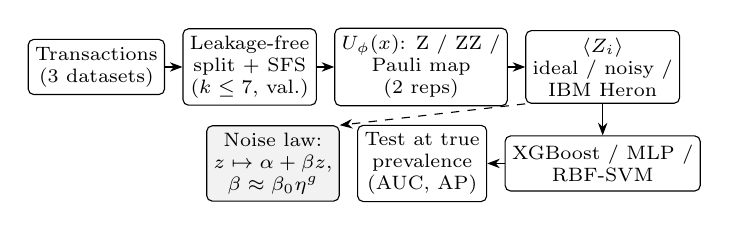
\begin{tikzpicture}[font=\scriptsize, node distance=2.2mm and 2.2mm,
  box/.style={draw, rounded corners=2pt, align=center, inner sep=2.5pt, minimum height=7mm},
  arr/.style={-{Stealth[length=1.6mm]}, thin}]
\node[box] (d) {Transactions\\(3 datasets)};
\node[box, right=of d] (s) {Leakage-free\\split + SFS\\($k\le7$, val.)};
\node[box, right=of s] (q) {$U_\phi(x)$: Z / ZZ /\\Pauli map\\(2 reps)};
\node[box, right=of q] (z) {$\langle Z_i\rangle$\\ideal / noisy /\\IBM Heron};
\node[box, below=4mm of z] (c) {XGBoost / MLP /\\RBF-SVM};
\node[box, left=of c] (e) {Test at true\\prevalence\\(AUC, AP)};
\node[box, left=of e, fill=black!5] (t) {Noise law:\\$z\mapsto\alpha+\beta z$,\\$\beta\approx\beta_0\eta^{g}$};
\draw[arr] (d)--(s); \draw[arr] (s)--(q); \draw[arr] (q)--(z); \draw[arr] (z)--(c); \draw[arr] (c)--(e);
\draw[arr, dashed] (z.south west)--(t.north east);
\end{tikzpicture}
\caption{Pipeline. Quantum expectation features of SFS-selected inputs are computed ideally, under two architecture noise models, or on IBM Heron hardware, and fed to classical classifiers; Section~IV characterizes how noise transforms them.}
\label{fig:pipeline}
\end{figure}

\subsection{Data and leakage-free protocol}
We use the European credit-card dataset~\cite{dalpozzolo2015} (real; 1,081 exact duplicate rows removed), PaySim~\cite{paysim2016} and BankSim~\cite{banksim2014} (synthetic, agent-based simulators calibrated on real logs). Identifiers and PaySim's rule-based \texttt{isFlaggedFraud} flag are dropped; BankSim's merchant is target-encoded out-of-fold on training rows only (Table~\ref{tab:data}). Each dataset is split 60/20/20 (stratified) with three seeds; all transformations are fitted on the training partition. Training rows are undersampled (30k rows, $\leq$50\% fraud). Validation and test partitions keep the \emph{original prevalence}; where genuine rows are subsampled (PaySim test), inverse-probability weights make every metric unbiased for the full partition. Hyper-parameters (6--8 configurations per classifier) and the decision threshold (max-F1) are chosen on validation; the test set is used once. We report weighted ROC-AUC and average precision (AP) with 200-sample Poisson-bootstrap CIs.

\begin{table}[t]
\centering
\caption{Datasets after cleaning (test partition at original prevalence).}
\label{tab:data}
\scriptsize
\setlength{\tabcolsep}{3pt}
\begin{tabular}{lrrrr}
\toprule
Dataset & Rows & Frauds (\%) & Feat. & Test rows (frauds)\\
\midrule
Credit card (real) & 283,726 & 473 (0.167) & 30 & 56,746 (95)\\
PaySim (synthetic) & 6,362,620 & 8,213 (0.129) & 12 & 1,272,524 (1,643)\\
BankSim (synthetic) & 594,643 & 7,200 (1.211) & 24 & 118,929 (1,440)\\
\bottomrule
\end{tabular}
\end{table}

\subsection{Feature selection (SFS)}
One qubit encodes one feature, so $k\le7$ features are selected by sequential forward selection on the \emph{validation} set, scoring the ideal quantum features of each candidate subset with a fixed logistic-regression evaluator. The full path to $k=7$ costs $\le$189 evaluations for 30 candidates (versus $\approx2.8\times10^6$ subsets of size $\le7$); the smallest subset within $10^{-4}$ AUC of the best is kept.

\subsection{Quantum features}
For $x\in[0,1]^k$ we use Qiskit~\cite{qiskit2024} \texttt{ZFeatureMap}, \texttt{ZZFeatureMap} (full entanglement) and \texttt{PauliFeatureMap} with Paulis $[Z,Y,ZZ]$, all with 2 repetitions, and read out $z_i(x)=\langle\psi(x)|Z_i|\psi(x)\rangle$. Inputs are mapped to angles in $[-1,1]$ (Z) or $[\pi-\sqrt{\pi},\pi]$ (ZZ, Pauli), a range in which every Qiskit phase term spans at most $2\pi$ and cannot wrap around. Ideal features are computed with an exact vectorized statevector simulator built from the transpiled circuits (agreement with Qiskit to $10^{-14}$). We also evaluate the classical features of the same SFS subset (``C-SFS'') and all classical features (``C-all'').

\subsection{Architectures, noise and shots}
Noisy features are computed with Qiskit Aer density-matrix simulation on paired subsets (18--21k rows per task). The \emph{superconducting} model uses a 7-qubit heavy-hex (Falcon-like) coupling map, basis $\{r_z,\sqrt{X},X,\mathrm{CX}\}$ with SWAP routing, $T_1{=}60\,\mu$s, $T_2{=}30\,\mu$s, gate times 60/550\,ns, depolarizing 0.04\%/2\% and 4\% readout error. The \emph{trapped-ion} model is all-to-all with native $\{r_x,r_y,r_z,R_{XX}\}$, depolarizing 0.06\%/0.5\%, amplitude/phase damping $5{\cdot}10^{-5}/3{\cdot}10^{-4}$ and 0.3\% readout. Readout error is applied exactly to the probability vector. A 2$\times$2 design (ideal/noisy $\times$ exact/1024 shots) separates gate noise from shot noise.

\subsection{IBM hardware protocol}
Seven jobs ran on the 156-qubit IBM Heron processors \texttt{ibm\_marrakesh} and \texttt{ibm\_fez} (247\,s of QPU time in total). Fixed, stratified subsets of the paired rows (1,689--1,800 rows: 800 train, 394--450 validation, 495--550 test) were embedded as 8--40 parallel copies of the $k$-qubit circuit on disjoint physical qubits, measured with 1,024 shots, \emph{without} any error mitigation, twirling or dynamical decoupling. The same rows were evaluated ideally and in both noise models, so all comparisons are row-paired. Classifiers are trained and tested on hardware features; in a \emph{transfer} setting, a model trained on ideal features is applied to hardware features after an affine calibration fitted on training rows only.

\section{Theory: an affine noise law for product maps}
Let $\mathcal{N}$ be the set of single-qubit channels acting on the Bloch vector $r$ as $r\mapsto(\lambda_\perp r_x,\lambda_\perp r_y,\lambda_\parallel r_z+\kappa)$. $\mathcal{N}$ is closed under composition and contains depolarizing ($\lambda_\perp{=}\lambda_\parallel{=}1{-}p$, $\kappa{=}0$), amplitude damping ($\sqrt{1-\gamma},1-\gamma,\gamma$), dephasing ($\sqrt{1-\lambda},1,0$) and thermal relaxation ($e^{-t/T_2},e^{-t/T_1},1-e^{-t/T_1}$). Every $\Phi\in\mathcal{N}$ commutes with $z$-rotations. Readout with flip probabilities $p_{01},p_{10}$ maps a measured $\ev{Z}$ to $\rho\ev{Z}+o$ with $\rho=1-p_{01}-p_{10}$.

\begin{proposition}[Affine noise law]
Let qubit $i$ of the 2-repetition Z feature map run $H,P(\phi_i),H,P(\phi_i)$ with $\phi_i=2\tilde x_i$, each gate followed by a channel in $\mathcal{N}$, and per-qubit readout error. Then for every input,
\begin{equation}
z_i^{\mathrm{noisy}}(x)=\alpha_i+\beta_i\,z_i^{\mathrm{ideal}}(x),\qquad z_i^{\mathrm{ideal}}=\cos\phi_i,
\end{equation}
with $\beta_i=\rho\,\lambda_\parallel^{(P_2)}\lambda_\parallel^{(H_2)}\lambda_\perp^{(P_1)}\lambda_\perp^{(H_1)}$ and $\alpha_i$ independent of $x$. Moreover $z_i^{\mathrm{noisy}}$ depends on $x_i$ only.
\end{proposition}
\begin{proof}
Track the Bloch vector of qubit $i$: $(0,0,1)\xrightarrow{H}(1,0,0)\xrightarrow{\Phi}(\lambda_\perp,0,\kappa)\xrightarrow{P(\phi)}(\lambda_\perp\cos\phi,\lambda_\perp\sin\phi,\kappa)$. The next channel scales the $x$ component by $\lambda_\perp^{(P_1)}$; $H$ maps $x\mapsto z$, giving $z=\lambda_\perp^{(P_1)}\lambda_\perp^{(H_1)}\cos\phi$; the subsequent channel gives $\lambda_\parallel^{(H_2)}z+\kappa^{(H_2)}$; $P(\phi)$ leaves $z$ unchanged; the last channel and the readout are affine in $z$. Without two-qubit gates, the reduced state of qubit $i$ depends on $\phi_i$ only.
\end{proof}
On the superconducting model, $H$ compiles to $R_z\sqrt{X}R_z$ with error-free virtual $R_z$; since $\Phi$ commutes with $R_z$, the noisy Hadamard is exactly $\Phi\circ H$ and $\beta=(1-2p_{\mathrm{ro}})e^{-t/T_1}e^{-t/T_2}(1-p_{1q})^2=0.91651$.

\begin{corollary}[Pipeline invariance]
If $\beta_i>0$, standardized features are identical with and without noise, $(\beta z+\alpha-\beta\mu-\alpha)/(\beta\sigma)=(z-\mu)/\sigma$. Every standardized model---the logistic SFS evaluator, MLP, RBF-SVM---and thus the selected subset, hyper-parameters, threshold and test metrics are unchanged; tree models are invariant to strictly increasing per-feature maps in exact arithmetic.
\end{corollary}
\begin{corollary}[Noise as a shot multiplier]
With $S$ shots, $\hat z=\alpha+\beta z+\varepsilon$, $\mathrm{Var}\,\varepsilon=(1-(\alpha+\beta z)^2)/S$. The calibrated estimate $(\hat z-\alpha)/\beta$ has the variance of an ideal estimate with $S_{\mathrm{eff}}\lesssim\beta^2S$ shots: noise multiplies the shot budget by $\approx1/\beta^2$.
\end{corollary}
With two-qubit gates, errors on one qubit propagate into others and $z_i^{\mathrm{noisy}}$ is no longer a function of $z_i^{\mathrm{ideal}}$ alone; the distortion is then neither exactly affine nor removable by calibration.

\section{Results}
\subsection{Does noise hurt quantum features? Not for product maps}
\textbf{Simulation.} For the Z map, the affine fit of noisy on ideal features has a maximum residual of $2.2\times10^{-15}$ for both architecture models at $1\times$, $3\times$ and $10\times$ baseline noise, and the fitted $\beta$ matches the closed form to $2\times10^{-15}$. On the real paired rows of all 18 Z-map tasks (3 datasets $\times$ 3 seeds $\times$ 2 architecture models) the residual is $6\times10^{-14}$. Retraining on noisy instead of ideal Z features changes test AUC by $1.0\times10^{-7}$ (logistic regression), $1.1\times10^{-7}$ (MLP) and $4.8\times10^{-7}$ (SVM), averaged over 9 tasks per model---no larger than a round-off control in which ideal features are perturbed by $10^{-12}$ ($1.2\times10^{-7}$, $1.4\times10^{-7}$, $3.2\times10^{-6}$). XGBoost shows $|\Delta\mathrm{AUC}|=2\times10^{-3}$, which we trace to its 32-bit histogram binning rather than to information loss. For entangling maps the same logistic test is not invariant: $|\Delta\mathrm{AUC}|=4\times10^{-6}$ (ZZ, trapped-ion), $2\times10^{-4}$ (ZZ, superconducting) and $3\times10^{-3}$ (Pauli, superconducting), ordered by their distance from the affine law (residuals $6\times10^{-4}$, $3\times10^{-2}$, $6\times10^{-2}$).

\textbf{Hardware.} Fig.~\ref{fig:affine}a shows measured versus ideal features for a representative (median-$\beta$) physical qubit. Fitting the affine law separately for every physical qubit (360 qubits over four Z-map jobs on two devices and three datasets; Table~\ref{tab:hw}), the median $R^2$ is 0.997 and the residual standard deviation is 1.08--1.11$\times$ the binomial shot-noise level: \emph{on real hardware, the Z map obeys Proposition~1 to within shot noise.} The per-qubit $\beta$ varies across the chip (median 0.96--0.98; a few defective qubits below 0.2), which a per-feature calibration absorbs. Classifiers trained and tested on hardware Z features match ideal features sampled with the same 1,024 shots on the same rows within $\pm0.012$ AUC in all 12 device$\times$dataset$\times$classifier pairs, with no systematic sign (Table~\ref{tab:hw}); the remaining gap to exact ideal features (up to 0.022 on BankSim) is shot noise. A model trained purely in simulation transfers to hardware after an affine calibration on credit card (AUC 0.938 vs.\ 0.931 ideal, XGBoost); on PaySim and BankSim the transfer loses 0.01--0.07 because our calibration was pooled over physical qubits whose $\beta$ differ, so per-qubit calibration is required.

\begin{figure*}[t]
\centering
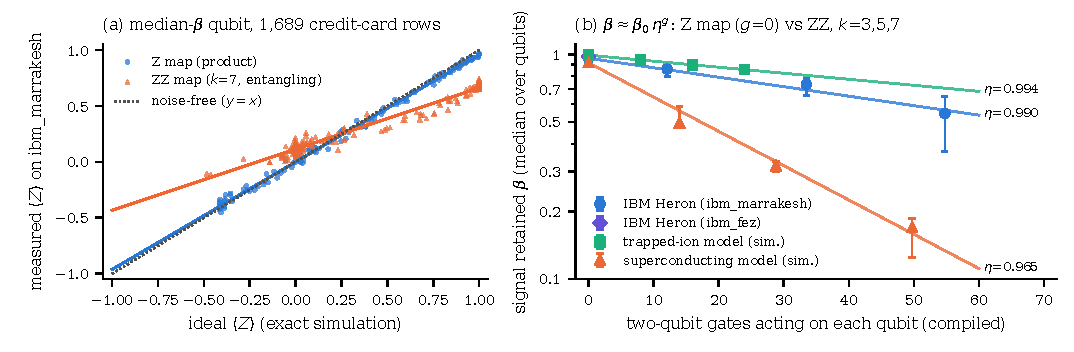
\includegraphics[width=\textwidth]{fig_affine_beta.pdf}
\caption{(a) Ideal vs.\ measured $\ev{Z}$ on \texttt{ibm\_marrakesh} for the median-$\beta$ qubit of each map: the product (Z) map lies on a line close to $y=x$; the entangling ZZ map ($k=7$) is compressed and scattered. (b) Signal retained $\beta$ (median and interquartile range over qubits) against compiled two-qubit gates per qubit $g$; lines are fits of $\beta=\beta_0\eta^{g}$ with $\beta_0$ the measured Z-map value. Hardware: Z map ($g{=}0$, two devices, three datasets) and ZZ with $k=3,5,7$ on the same credit-card rows.}
\label{fig:affine}
\end{figure*}

\begin{table*}[t]
\centering
\caption{IBM Heron hardware runs (1,024 shots, no error mitigation). $g$: compiled two-qubit gates per qubit; $\beta$, $R^2$: medians of per-qubit affine fits of hardware on ideal features; $r/\sigma$: residual s.d.\ over expected shot-noise s.d. AUC on the hardware test rows (XGBoost / SVM / MLP) vs.\ ideal features of the same rows sampled with the same 1,024 shots.}
\label{tab:hw}
\scriptsize
\begin{tabular}{llcrrcccccc}
\toprule
Dataset & Device & Map, $k$ & $g$ & Qubits & $\beta$ & $R^2$ & $r/\sigma$ & AUC hardware & AUC ideal, 1,024 shots & QPU [s]\\
\midrule
Credit card & marrakesh & Z, 7 & 0 & 98 & 0.961 & 0.997 & 1.10 & 0.949 / 0.938 / 0.938 & 0.937 / 0.938 / 0.934 & 36\\
Credit card & fez & Z, 7 & 0 & 98 & 0.976 & 0.997 & 1.08 & 0.940 / 0.941 / 0.937 & 0.937 / 0.938 / 0.934 & 34\\
PaySim & marrakesh & Z, 6 & 0 & 84 & 0.959 & 0.996 & 1.10 & 0.979 / 0.974 / 0.978 & 0.985 / 0.976 / 0.983 & 38\\
BankSim & marrakesh & Z, 2 & 0 & 80 & 0.960 & 0.997 & 1.11 & 0.975 / 0.953 / 0.961 & 0.965 / 0.960 / 0.955 & 15\\
\midrule
Credit card & marrakesh & ZZ, 3 & 12.1 & 75 & 0.859 & 0.992 & 1.54 & 0.915 / 0.904 / 0.922 & 0.933 / 0.922 / 0.945 & 21\\
Credit card & marrakesh & ZZ, 5 & 33.5 & 70 & 0.734 & 0.984 & 1.40 & 0.919 / 0.927 / 0.924 & 0.942 / 0.935 / 0.938 & 37\\
Credit card & marrakesh & ZZ, 7 & 54.8 & 56 & 0.544 & 0.963 & 1.37 & 0.922 / 0.919 / 0.892 & 0.936 / 0.919 / 0.917 & 66\\
\bottomrule
\end{tabular}
\end{table*}

\subsection{What does entanglement cost? A geometric signal decay}
The ZZ map loses signal with every two-qubit gate. On hardware, the median $\beta$ falls from 0.96 (Z, $g{=}0$) to 0.86, 0.73 and 0.54 for $k=3,5,7$ ($g=12,34,55$), a clean geometric decay with $\eta=0.990$ per two-qubit gate per qubit (Fig.~\ref{fig:affine}b). The simulated architectures follow the same law with $\eta=0.994$ (trapped-ion) and $0.965$ (superconducting); the latter is pessimistic relative to Heron. Connectivity enters through $g$: compiling the 7-qubit ZZ map needs 84 two-qubit gates all-to-all, 174 on the Falcon-like map (90 from routing) and 192 per copy on Heron. Unlike the Z map, the ZZ map loses accuracy relative to equally-shot ideal features on hardware ($-0.008$ to $-0.025$ AUC in 8 of 9 classifier$\times k$ pairs, Table~\ref{tab:hw}), and transferring an ideal-trained model to ZZ hardware features after affine calibration costs up to 0.056 AUC on credit card, where the same transfer is lossless for the Z map.

Corollary~2 turns $\beta$ into measurement cost (Fig.~\ref{fig:shots}). With the Z map, the ideal, trapped-ion and superconducting curves coincide within seed variability, as predicted by $1/\beta^2\le1.19$; on credit card the AUC is within 0.005 of its exact-expectation value from 16--64 shots. The entangling maps on the superconducting model need 2,048--4,096 shots (credit card and BankSim, ZZ and Pauli) or do not get within 0.005 AUC by 8,192 shots, whereas the trapped-ion model needs 32--256 shots on credit card and BankSim. At 64 shots, PaySim-ZZ reaches AUC 0.810 (superconducting) vs.\ 0.967 (trapped-ion). On hardware, re-using the first $S$ of the recorded shots, the Z map is within 0.01 AUC of its 1,024-shot value from 32 shots, while ZZ ($k{=}7$) drops to 0.81 at 16 and 0.89 at 64 shots against 0.94 for ideal features on the same rows.

\begin{figure*}[t]
\centering
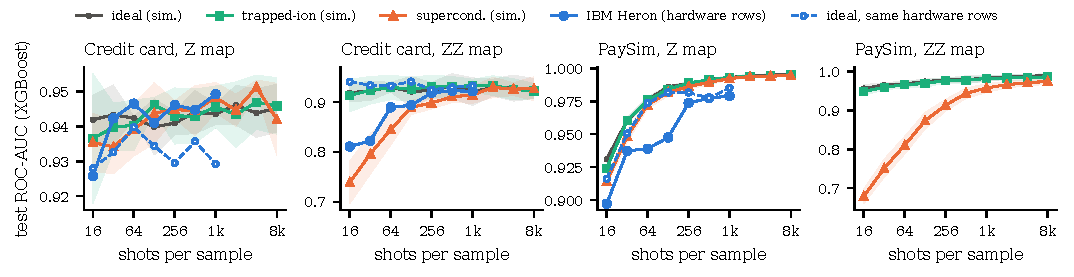
\includegraphics[width=\textwidth]{fig_shots.pdf}
\caption{Test ROC-AUC (XGBoost) vs.\ shots per sample. Simulation curves: mean $\pm$ s.d.\ over three seeds on the paired rows. Hardware curves (credit card, PaySim) use the first $S$ recorded shots of the IBM runs and are compared with ideal features on the same, smaller row set (dashed).}
\label{fig:shots}
\end{figure*}

\subsection{Does it pay for fraud detection? No}
\begin{table*}[t]
\centering
\caption{Test ROC-AUC (average precision) at original prevalence, mean over three seeds. Quantum columns: ideal $\ev{Z_i}$ features of the SFS-selected $k\le7$ inputs.}
\label{tab:main}
\scriptsize
\begin{tabular}{llcccc}
\toprule
Dataset & Classifier & Classical, all features & Quantum, Z map & Quantum, ZZ map & Quantum, Pauli map\\
\midrule
\multirow{3}{*}{Credit card} & XGBoost & \textbf{0.967} (0.762) & 0.940 (0.628) & 0.923 (0.585) & 0.951 (0.602)\\
 & MLP & \textbf{0.959} (0.734) & 0.936 (0.524) & 0.921 (0.540) & 0.924 (0.506)\\
 & SVM & \textbf{0.971} (0.593) & 0.926 (0.312) & 0.891 (0.107) & 0.932 (0.145)\\
\midrule
\multirow{3}{*}{PaySim} & XGBoost & \textbf{1.000} (0.934) & 0.999 (0.857) & 0.997 (0.801) & 0.998 (0.805)\\
 & MLP & \textbf{1.000} (0.941) & 0.997 (0.790) & 0.996 (0.711) & 0.998 (0.767)\\
 & SVM & \textbf{0.999} (0.946) & 0.990 (0.354) & 0.981 (0.395) & 0.988 (0.320)\\
\midrule
\multirow{3}{*}{BankSim} & XGBoost & \textbf{0.998} (0.894) & 0.971 (0.630) & \textbf{0.998} (0.881) & 0.997 (0.882)\\
 & MLP & \textbf{0.998} (0.899) & 0.970 (0.623) & 0.997 (0.844) & 0.997 (0.843)\\
 & SVM & 0.994 (0.603) & 0.958 (0.323) & \textbf{0.996} (0.764) & 0.995 (0.775)\\
\bottomrule
\end{tabular}
\end{table*}

Table~\ref{tab:main} compares ideal quantum features with all classical features. Quantum features of $k\le7$ selected inputs come close in ROC-AUC on the synthetic datasets but trail in AP and on the real credit-card data. Against the \emph{same} selected inputs used classically, the mean AUC difference is $-0.019$ (credit card), $-0.005$ (PaySim) and $-0.003$ (BankSim); quantum features win in at least two of three seeds in only 4 of 27 dataset$\times$map$\times$classifier settings. The one notable gain---the RBF-SVM on BankSim with ZZ/Pauli features (AP 0.76--0.78 vs.\ 0.55--0.60)---is a property of the kernel model, not of the data: XGBoost reaches AP 0.88 on either representation.

\textbf{Hybrid test with a classical control.} Appending the $k$ quantum features to all classical features (paired bootstrap, 500 resamples, same test rows) changes AUC by at most $+0.008$ in all 27 settings. Significant gains in all three seeds occur only for the RBF-SVM on BankSim (ZZ/Pauli: $+0.001$ AUC, $+0.095$ AP); appending $k$ \emph{random Fourier features} of the same inputs gives the same or larger gains ($+0.096$ to $+0.139$ AP), and quantum features beat this control in AUC in at most one seed of any setting.

\textbf{Fidelity-kernel QSVM.} As a reference, a fidelity-kernel QSVM trained on 2,000 rows reaches AUC 0.920--0.998, within 0.025 of an RBF-SVM on the same raw inputs, which is better in 6 of 9 dataset$\times$map settings, at up to 244\,s of kernel computation per fit versus under a second.

\subsection{Feature selection and silent pitfalls}
SFS against exhaustive search on a 10-feature pool ($k\le4$; credit card and BankSim; 72 comparisons) finds the exact optimum in 75\% of cases with a mean validation-AUC gap of 0.001 (max 0.024, ZZ) using 34 instead of 385 evaluations. We also found three silent failure modes that affect published pipelines: (i) with one repetition, $\ev{Z_i}\equiv0$ for all three maps, because a Hadamard layer followed by diagonal phase gates leaves every computational-basis marginal at $1/2$, so expectation features require $\ge2$ repetitions; (ii) Qiskit's \texttt{PauliFeatureMap} with $[X,ZZ]$ yields exactly the Z-basis statistics of \texttt{ZZFeatureMap}, so the two are not independent design choices; (iii) inputs scaled to $[-1,1]$ make the ZZ phase $(\pi-x_i)(\pi-x_j)$ wrap around $2\pi$ several times, scrambling neighbouring inputs. Selecting features or reporting results on a balanced or re-used test set inflates reported AUCs; all our numbers are on untouched test sets at the true prevalence.

\section{Discussion}
\textbf{A design rule.} For expectation-value features on current hardware, use product maps and spend the shot budget on data, not on entanglement. With Heron's $\eta\approx0.99$, keeping $\beta\ge0.5$ allows only $g\approx65$ two-qubit gates per qubit; a fully connected 7-qubit ZZ map with two repetitions already uses 55 on heavy-hex hardware. Each halving of $\beta$ quadruples the shots needed (Corollary~2), and our accuracy results show that entanglement bought no accuracy in return.

\textbf{The robustness--expressivity tension.} The product map's ideal feature is $\cos\phi_i$, a classical function of one input, and its noise immunity follows from exactly this structure. The maps that could carry non-classical correlations are the ones whose signal hardware erodes geometrically. This mirrors the trainability--simulability argument of~\cite{cerezo2025} for feature extraction, and explains why our hybrid gains vanish against a matched classical control: on today's hardware, the quantum features that survive noise are the ones a classical computer already provides.

\textbf{Limitations.} We use $k\le7$ qubits, IBM-style and trapped-ion-style noise \emph{models} rather than ion hardware, and small hardware test sets (95--150 frauds; CIs $\pm0.03$ AUC). The entangling-depth scan uses one dataset and one device. Hardware runs used no error mitigation, by design; mitigation would raise $\beta$ but cannot undo non-affine mixing. Proposition~1 covers phase-covariant single-qubit noise; coherent errors and crosstalk are only tested empirically (on hardware, residuals stayed at the shot-noise level for product maps).

\section{Conclusion}
For fraud detection with quantum expectation features, noise is harmless for product maps---provably, in simulation, and on two IBM Heron processors---and costly for entangling maps, whose signal decays by about 1\% per two-qubit gate per qubit on current hardware. Since no quantum representation outperformed classical features on three datasets, the practical recommendation is clear: entanglement in feature maps pays only if it buys accuracy that classical features cannot, and the per-gate cost law $\beta\approx\beta_0\eta^{g}$ quantifies how good hardware must become before that is even testable. Code and all result files will be released upon acceptance.

\bibliographystyle{IEEEtran}
\begin{thebibliography}{99}
\bibitem{havlicek2019} V. Havl\'{\i}\v{c}ek, A. D. C\'orcoles, K. Temme, A. W. Harrow, A. Kandala, J. M. Chow, and J. M. Gambetta, ``Supervised learning with quantum-enhanced feature spaces,'' \emph{Nature}, vol. 567, pp. 209--212, 2019.
\bibitem{schuld2019} M. Schuld and N. Killoran, ``Quantum machine learning in feature Hilbert spaces,'' \emph{Phys. Rev. Lett.}, vol. 122, p. 040504, 2019.
\bibitem{grossi2022} M. Grossi, N. Ibrahim, V. Radescu, R. Loredo, K. Voigt, C. von Altrock, and A. Rudnik, ``Mixed quantum--classical method for fraud detection with quantum feature selection,'' \emph{IEEE Trans. Quantum Eng.}, vol. 3, pp. 1--12, 2022.
\bibitem{bowles2024} J. Bowles, S. Ahmed, and M. Schuld, ``Better than classical? The subtle art of benchmarking quantum machine learning models,'' arXiv:2403.07059, 2024.
\bibitem{wang2021kernels} X. Wang, Y. Du, Y. Luo, and D. Tao, ``Towards understanding the power of quantum kernels in the NISQ era,'' \emph{Quantum}, vol. 5, p. 531, 2021.
\bibitem{heyraud2022} V. Heyraud, Z. Li, Z. Denis, A. Le Boit\'e, and C. Ciuti, ``Noisy quantum kernel machines,'' \emph{Phys. Rev. A}, vol. 106, p. 052421, 2022.
\bibitem{thanasilp2024} S. Thanasilp, S. Wang, M. Cerezo, and Z. Holmes, ``Exponential concentration in quantum kernel methods,'' \emph{Nat. Commun.}, vol. 15, 2024, doi:10.1038/s41467-024-49287-w.
\bibitem{huang2021} H.-Y. Huang, M. Broughton, M. Mohseni, R. Babbush, S. Boixo, H. Neven, and J. R. McClean, ``Power of data in quantum machine learning,'' \emph{Nat. Commun.}, vol. 12, p. 2631, 2021.
\bibitem{cerezo2025} M. Cerezo, M. Larocca, D. Garc\'{\i}a-Mart\'{\i}n, N. L. Diaz, P. Braccia, E. Fontana, M. S. Rudolph, P. Bermejo, A. Ijaz, S. Thanasilp, E. R. Anschuetz, and Z. Holmes, ``Does provable absence of barren plateaus imply classical simulability?'' \emph{Nat. Commun.}, vol. 16, p. 7907, 2025.
\bibitem{dalpozzolo2015} A. Dal Pozzolo, O. Caelen, R. A. Johnson, and G. Bontempi, ``Calibrating probability with undersampling for unbalanced classification,'' in \emph{Proc. IEEE Symp. Series on Computational Intelligence (SSCI)}, 2015.
\bibitem{paysim2016} E. A. Lopez-Rojas, A. Elmir, and S. Axelsson, ``PaySim: A financial mobile money simulator for fraud detection,'' in \emph{Proc. 28th European Modeling and Simulation Symp. (EMSS)}, 2016.
\bibitem{banksim2014} E. A. Lopez-Rojas and S. Axelsson, ``BankSim: A bank payments simulator for fraud detection research,'' in \emph{Proc. 26th European Modeling and Simulation Symp. (EMSS)}, 2014.
\bibitem{qiskit2024} A. Javadi-Abhari \emph{et al.}, ``Quantum computing with Qiskit,'' arXiv:2405.08810, 2024.
\end{thebibliography}

\end{document}
